% THIS TEMPLATE IS A WORK IN PROGRESS

\documentclass[polish, a4paper]{article}
\usepackage[a4paper,left=3cm,right=3cm,top=3cm,bottom=1.5cm]{geometry}
\usepackage[T1]{fontenc}
\usepackage[polish]{babel}
\usepackage[utf8]{inputenc}
\usepackage{hyperref}
\usepackage{fancyhdr}
\usepackage{float}
\usepackage{graphicx}
\usepackage{titling}
\usepackage{wasysym}
\usepackage{caption}
\usepackage{pgfplots}
\usepackage{pgfplotstable}
\usepackage{filecontents}
\usepackage{csvsimple}
\usepackage{textcomp}
\usepackage{gensymb}
\usepackage{etoolbox}
%\usepackage{siunitx}
\graphicspath{ {./} }
\pagestyle{fancy}

\setlength{\droptitle}{-1in}

%\lhead{\includegraphics[width=0.2\textwidth]{nyush-logo.pdf}}

  \lhead{Maciej Kaszkowiak}
  \chead{Podstawowe narzędzia sieciowe w Linuksie}
  \rhead{
  151856}


%%%% PROJECT TITLE
\title{Podstawowe narzędzia sieciowe w Linuksie \\
        \Large \emph{Sprawozdanie nr 2 z przedmiotu Sieci Komputerowe}}

%%%% NAMES OF ALL THE STUDENTS INVOLVED (first-name last-name)
\author{Maciej Kaszkowiak, 151856, zadania wykonane 1 kwietnia 2023}

\date{\vspace{-5ex}} %NO DATE


\begin{document}


\maketitle
%\thispagestyle{titlepage}

\tableofcontents

\newpage

\section{Zadanie 1}
Poniższe polecenia wykonywane są na interfejsie br0.

\subsection{Wspólnie z koleżankami/kolegami z rzędu ustal adres sieci, który pozwoli na zaadresowanie wszytkich komputerów w rzędzie. Sieci są unikalne między rzędami.}

\begin{verbatim}
192.168.X.Y, gdzie X to nr rzędu, zaś Y to nr komputera
192.168.1.0 / 24
\end{verbatim}
\subsection{Przypisz jeden z adresów do interfejsu em1 (każdy komputer w rzędzie ma mieć inny adres).}

\begin{verbatim}
lab-sec-3:/homex/student # ip addr add 192.168.1.3/24 dev br0
\end{verbatim}

\subsection{Przeanalizuj ruch na interfejsie em1 przy pomocy programu wireshark.}

\begin{figure}[H]
\centering
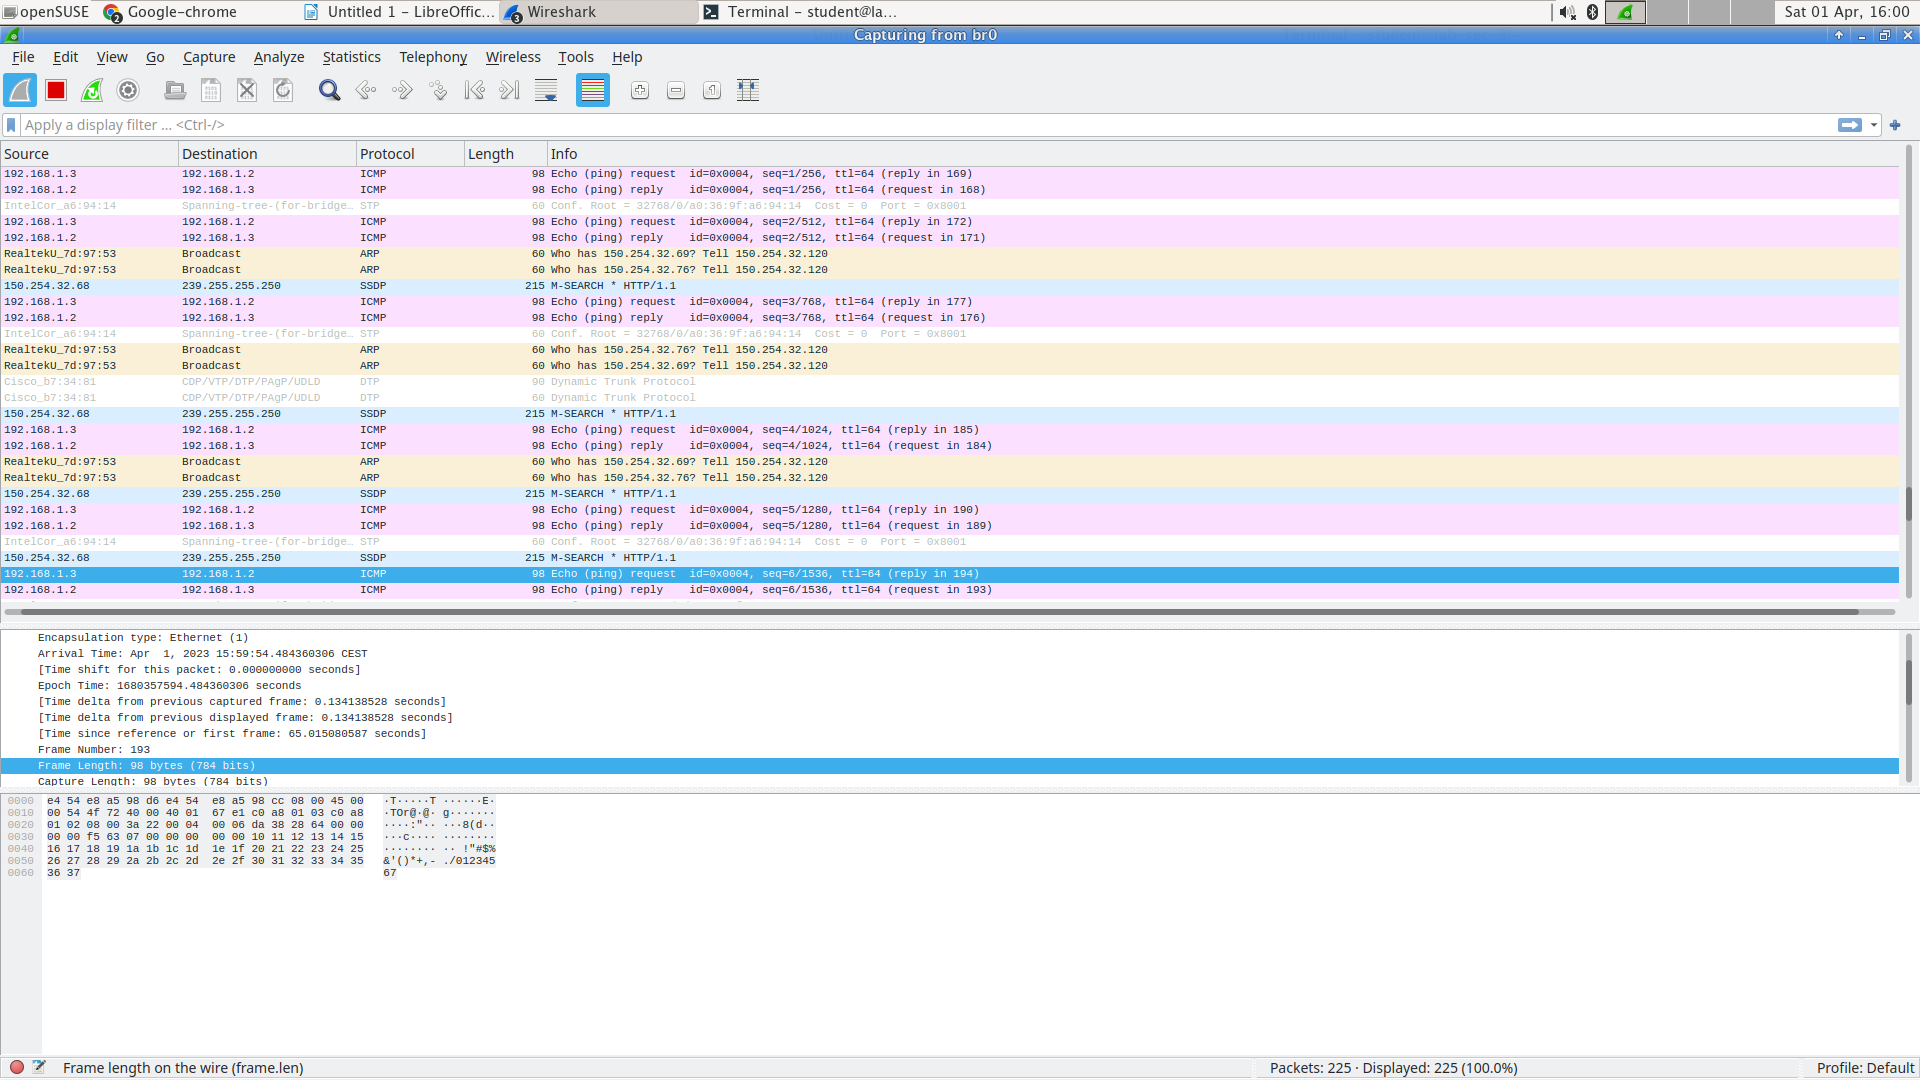
\includegraphics[width=\textwidth]{zdj1.png}
\caption{Ruch na interfejsie br0.}
\end{figure}

\subsection{Zbadaj przy pomocy polecenia ping połączenie z innymi komputerami w rzędzie.}

\begin{verbatim}
lab-sec-3:/homex/student # ping 192.168.1.2
PING 192.168.1.2 (192.168.1.2) 56(84) bytes of data.
64 bytes from 192.168.1.2: icmp_seq=1 ttl=64 time=0.545 ms
64 bytes from 192.168.1.2: icmp_seq=2 ttl=64 time=0.525 ms
64 bytes from 192.168.1.2: icmp_seq=3 ttl=64 time=0.556 ms
^C
--- 192.168.1.2 ping statistics ---
\end{verbatim}

Połączenie z innym komputerem w rzędzie działa.

\subsection{Zbadaj przy pomocy polecenia ping połączenie komputerami w innych rzędach.}

\begin{verbatim}
lab-sec-3:/homex/student # ping 192.168.2.5
PING 192.168.2.5 (192.168.2.5) 56(84) bytes of data.
From 150.254.4.66 icmp_seq=33 Destination Net Unreachable
From 150.254.4.66 icmp_seq=34 Destination Net Unreachable
\end{verbatim}

Połączenie z komputerami w pozostałych rzędach jest przy obecnej konfiguracji jest niewykonalne, ponieważ utworzyliśmy . Można wykonać połączenie za pomocą obecnie skonfigurowanego adresu IP:

\begin{verbatim}
lab-sec-3:/homex/student # ping 150.254.32.70
PING 150.254.32.70 (150.254.32.70) 56(84) bytes of data.
64 bytes from 150.254.32.70: icmp_seq=1 ttl=64 time=0.938 ms
64 bytes from 150.254.32.70: icmp_seq=2 ttl=64 time=0.370 ms
64 bytes from 150.254.32.70: icmp_seq=3 ttl=64 time=0.613 ms
64 bytes from 150.254.32.70: icmp_seq=4 ttl=64 time=0.620 ms
64 bytes from 150.254.32.70: icmp_seq=5 ttl=64 time=0.618 ms
64 bytes from 150.254.32.70: icmp_seq=6 ttl=64 time=0.730 ms
\end{verbatim}


\subsection{Parami połącz się z innym komputerem z rzędu przy pomocy komendy telnet i zbadaj treść wymienianych pakietów.}

\begin{verbatim}
lab-sec-3:/homex/student # telnet 192.168.1.2
Trying 192.168.1.2...
Connected to 192.168.1.2.
Escape character is '^]'.

Linux 5.14.21-150400.24.46-default (lab-sec-2) (2)

lab-sec-2 login: student
Password: 
Last login: Sat Apr  1 16:04:22 CEST 2023 from ::ffff:192.168.1.3 on pts/1
Last login: Sat Apr  1 16:07:59 from ::ffff:192.168.1.3
Have a lot of fun...
student@lab-sec-2:~> whoami
student
\end{verbatim}

\begin{figure}[H]
\centering
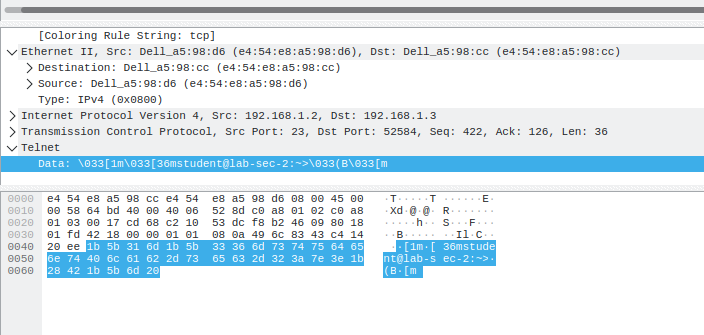
\includegraphics[width=\textwidth]{zdj2.png}
\caption{Zawartość pakietu telnet.}
\end{figure}

\begin{figure}[H]
\centering
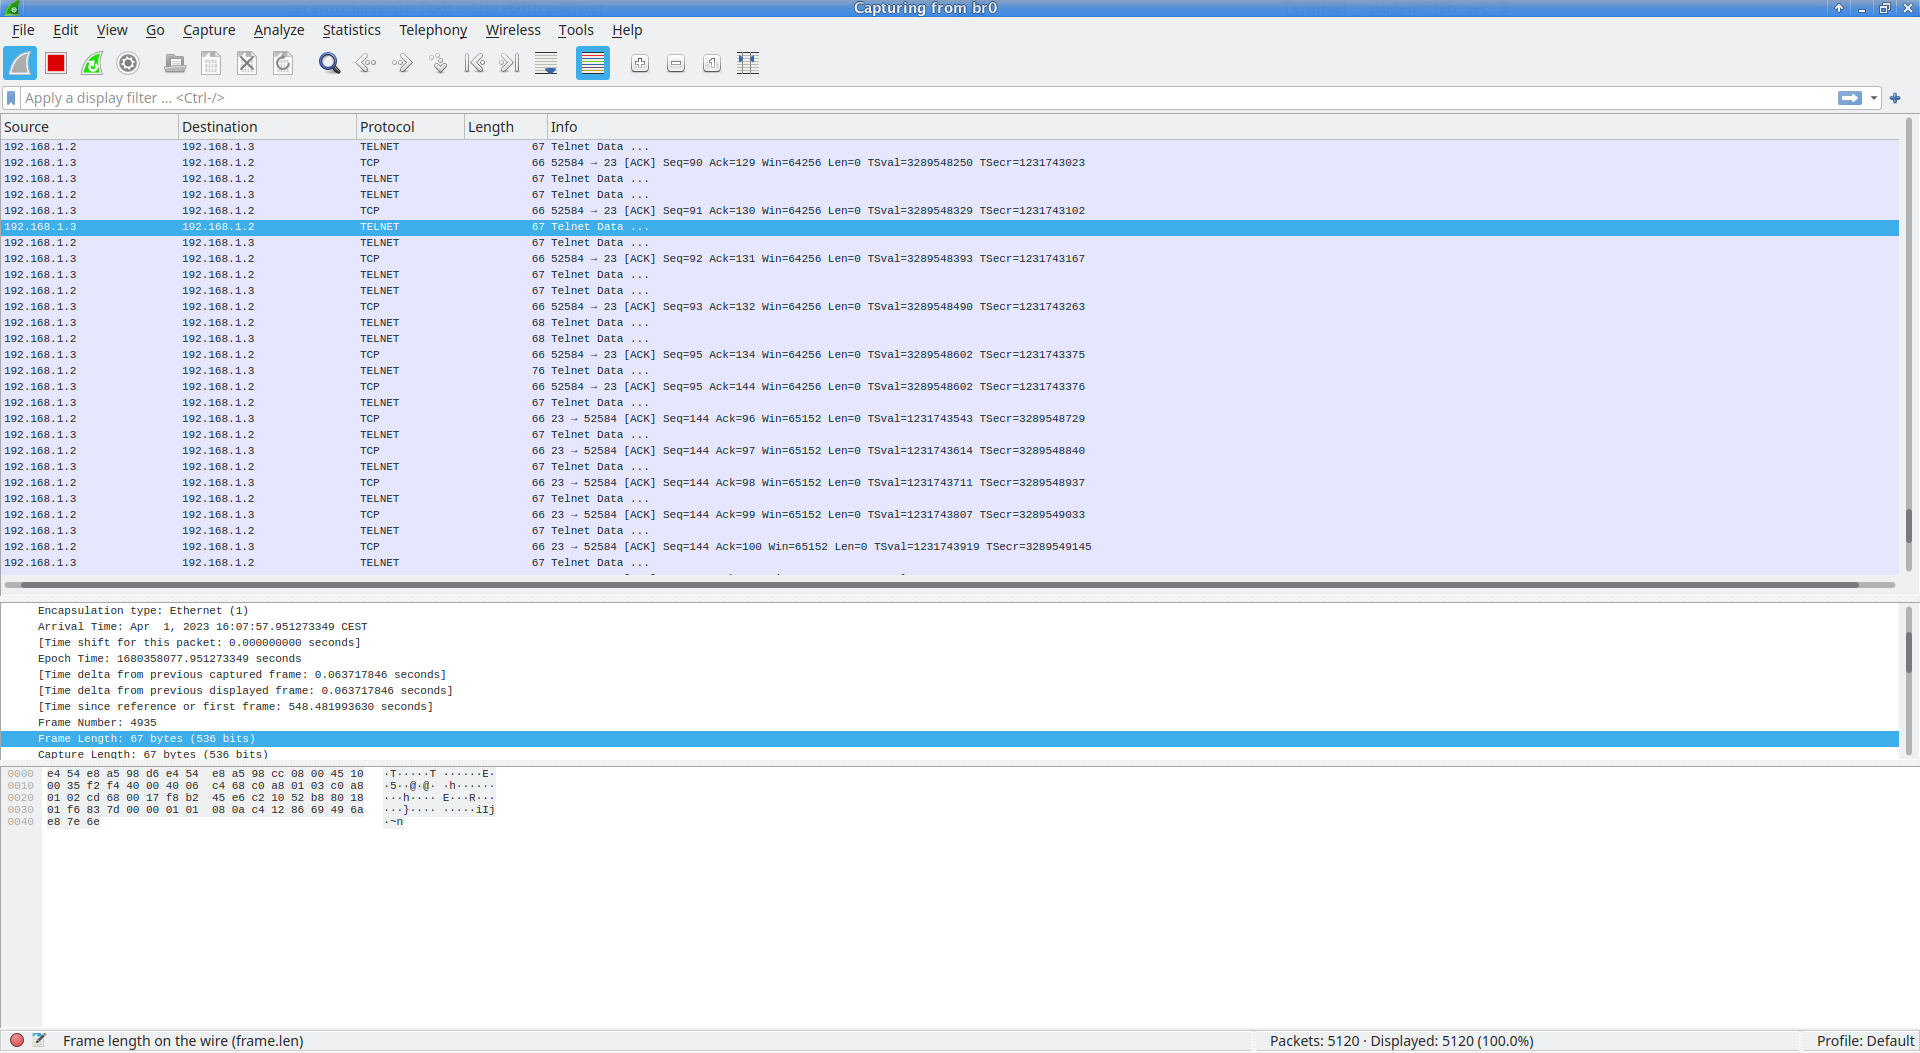
\includegraphics[width=\textwidth]{zdj3.png}
\caption{Wyniki pomiaru prędkości}
\end{figure}

Możemy zauważyć, że telnet przesyła nieszyfrowane dane, które z łatwością możemy odczytać za pomocą programu Wireshark.


\section{Zadanie 2}

W zadaniu pracuję na interfejsie em2.

\subsection{Zmierz osiąganą maksymalną prędkość transmisji przy użyciu
usługi speedtest.net.}

\begin{figure}[H]
\centering
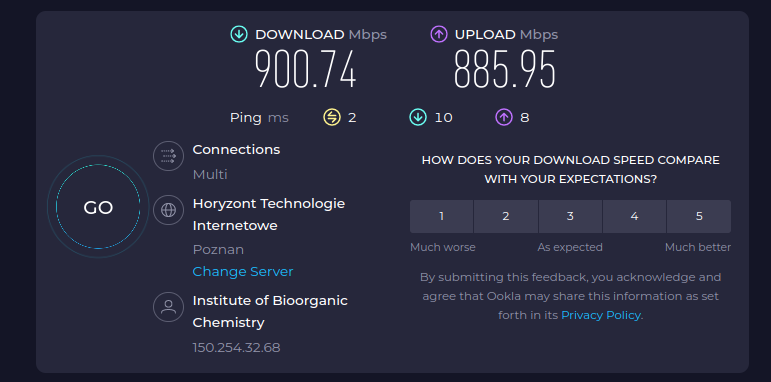
\includegraphics[width=0.7\textwidth]{speedtest1.png}
\caption{Wyniki pomiaru prędkości}
\end{figure}

Aktualnie interfejs ustawiony jest w tryb pełnego dupleksu przy prędkości 1000 Mb/s.

\begin{verbatim}

lab-sec-3:/homex/student # ethtool em2
Settings for em2:
	Supported ports: [ TP ]
	Supported link modes:   10baseT/Half 10baseT/Full
	                        100baseT/Half 100baseT/Full
	                        1000baseT/Full
	Supported pause frame use: No
	Supports auto-negotiation: Yes
	Supported FEC modes: Not reported
	Advertised link modes:  10baseT/Half 10baseT/Full
	                        100baseT/Half 100baseT/Full
	                        1000baseT/Full
	Advertised pause frame use: No
	Advertised auto-negotiation: Yes
	Advertised FEC modes: Not reported
	Speed: 1000Mb/s
	Duplex: Full
	Auto-negotiation: on
	Port: Twisted Pair
	PHYAD: 2
	Transceiver: internal
	MDI-X: off (auto)
	Supports Wake-on: pumbg
	Wake-on: g
        Current message level: 0x00000007 (7)
                               drv probe link
	Link detected: yes

\end{verbatim}


\subsection{Zmień parametry em1 ograniczając prędkość transmisji i
zmieniając parametry dupleksu.}

Modyfikuję prędkość interfejsu do 10 Mb/s w trybie pół-dupleksowym.
\begin{verbatim}
    lab-sec-3:/homex/student # ethtool -s em2 speed 10 duplex half
\end{verbatim}

\subsection{Ponownie zmierz maksymalną prędkość transmisji. Wróć do pierwotnych ustawień. Przy pomocy odpowiedniego parametru komendy ethtool
zidentyfikuj interfejsy p4p1 oraz p4p2.}

Możemy zaobserwować znaczący spadek:

\begin{figure}[H]
\centering
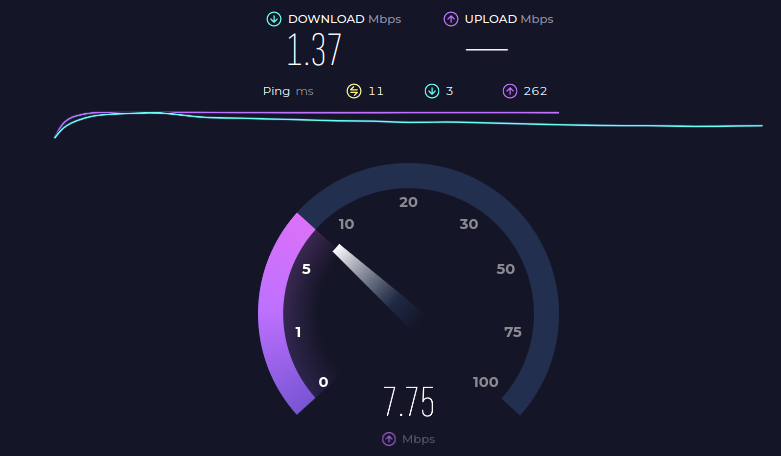
\includegraphics[width=0.7\textwidth]{speedtest2.png}
\caption{Wyniki pomiaru prędkości}
\end{figure}

Przywracam ustawienia interfejsu:

\begin{verbatim}
    lab-sec-3:/homex/student # ethtool -s em2 speed 1000 duplex full
\end{verbatim}

\begin{verbatim}
    lab-sec-3:/homex/student # ethtool -p p4p1
\end{verbatim}

\section{Zadanie 3}
\subsection{Usuń nadane wcześniej adresy IP na em1 (mają pozostać tylko
standardowe adresy, tj. uzyskiwane przez DHCP).}

Usuwam wcześniej nadany adres IP:

\begin{verbatim}
    lab-sec-3:/homex/student # ip address del 192.168.1.3/24 dev br0
\end{verbatim}

\subsection{Podłącz swój komputer poprzez port p4p1 do przełącznika na
zapleczu (wszystkie komputery są podłączane do tego samego
przełącznika).}

Podłączyłem swój komputer pod portem nr 99 pod switch, poprzez port p4p1.

\subsection{Skonfiguruj adres IP na porcie p4p1, tak by wszystkie
komputery w laboratorium mogły komunikować się między
sobą poprzez nowo utworzoną sieć}

Wykonałem następującą komendę:

\begin{verbatim}
    lab-sec-3:/homex/student # ip addr add 192.168.1.3/16 dev p4p1
\end{verbatim}

Komunikacja działa zarówno w obrębie rzędu jak i sali:

\begin{verbatim}
    lab-sec-3:/homex/student # ip addr add 192.168.1.3/16 dev p4p1
lab-sec-3:/homex/student # ping 192.168.1.2
PING 192.168.1.2 (192.168.1.2) 56(84) bytes of data.
64 bytes from 192.168.1.2: icmp_seq=1 ttl=64 time=0.549 ms
64 bytes from 192.168.1.2: icmp_seq=2 ttl=64 time=0.714 ms
64 bytes from 192.168.1.2: icmp_seq=3 ttl=64 time=0.250 ms
^C
--- 192.168.1.2 ping statistics ---
3 packets transmitted, 3 received, 0% packet loss, time 2040ms
rtt min/avg/max/mdev = 0.250/0.504/0.714/0.192 ms
lab-sec-3:/homex/student # ping 192.168.2.5
PING 192.168.2.5 (192.168.2.5) 56(84) bytes of data.
64 bytes from 192.168.2.5: icmp_seq=1 ttl=64 time=0.757 ms
64 bytes from 192.168.2.5: icmp_seq=2 ttl=64 time=0.706 ms
64 bytes from 192.168.2.5: icmp_seq=3 ttl=64 time=0.693 ms
^C
--- 192.168.2.5 ping statistics ---
3 packets transmitted, 3 received, 0% packet loss, time 2056ms
rtt min/avg/max/mdev = 0.693/0.718/0.757/0.027 ms

\end{verbatim}

Możemy zaobserwować komunikację w obrębie sieci, m.in. protokół ARP:

\begin{figure}[H]
\centering
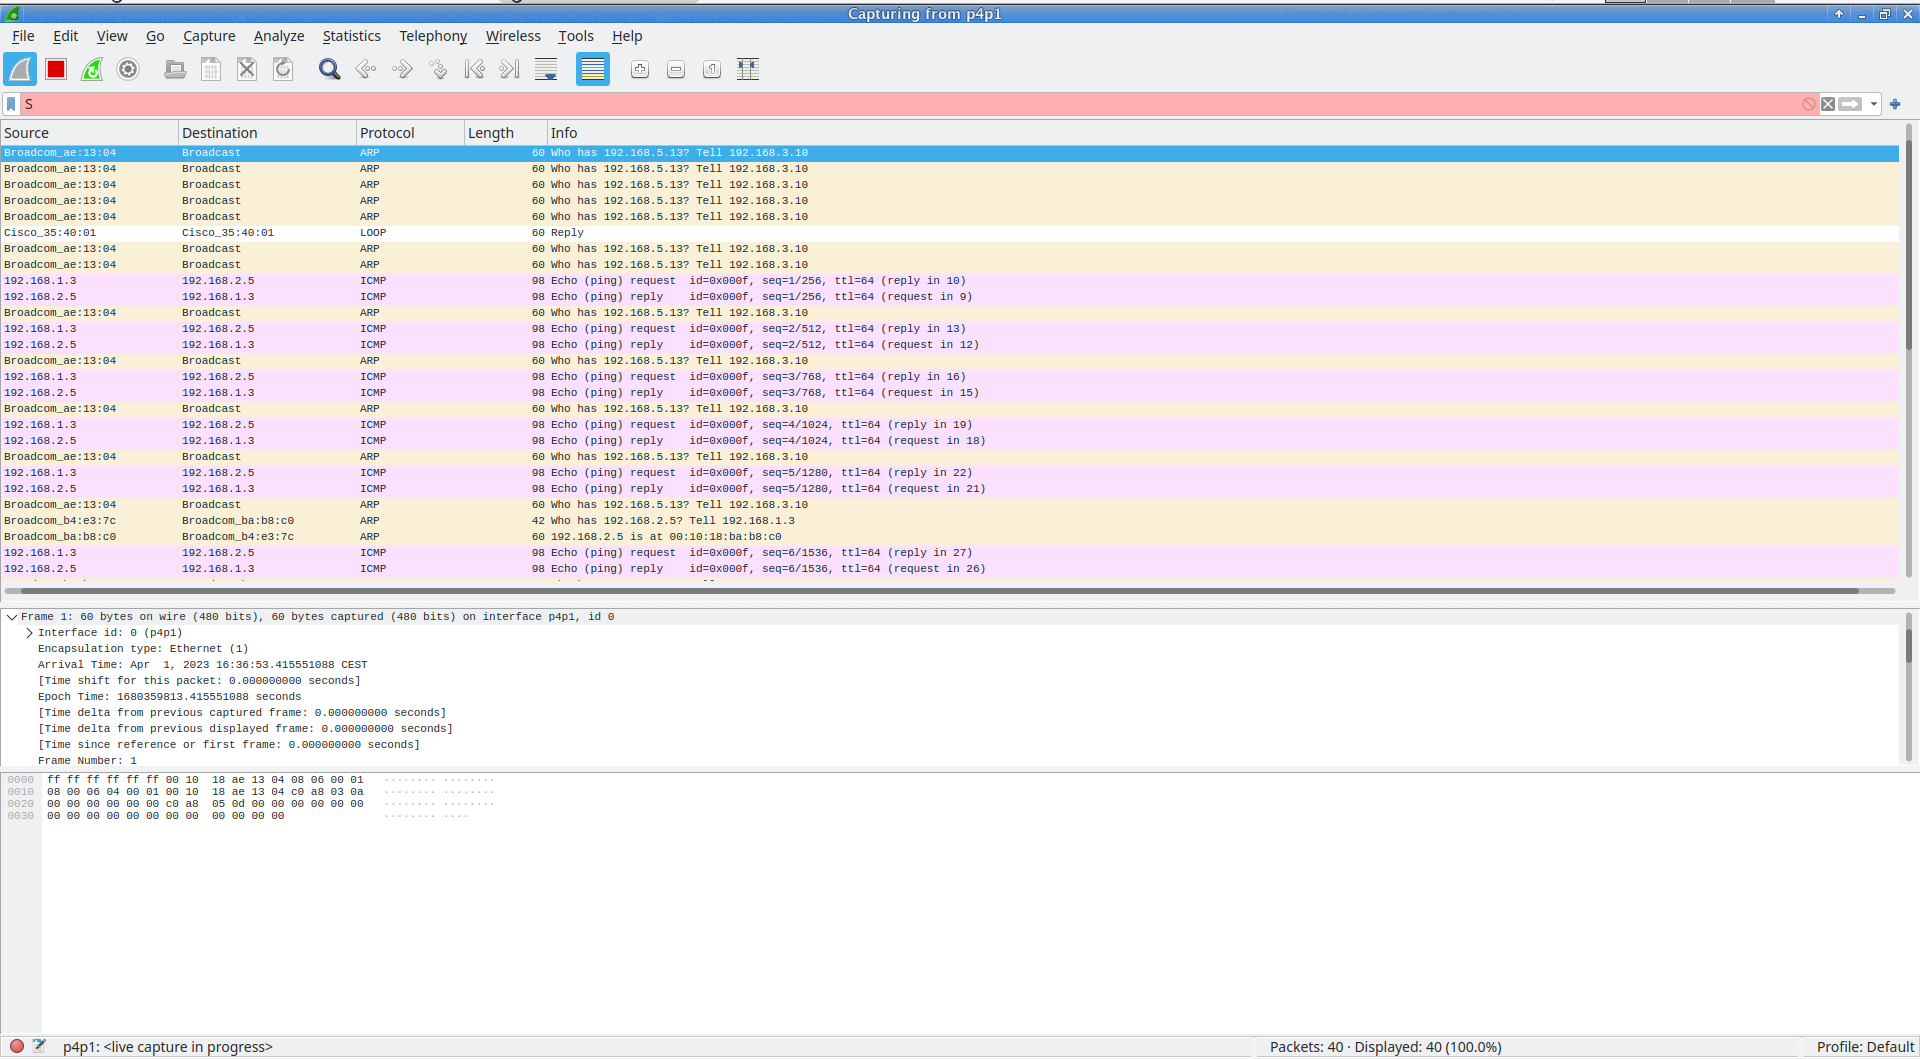
\includegraphics[width=\textwidth]{p4p1.png}
\caption{Wyniki pomiaru prędkości}
\end{figure}
\end{document}
